% Options for packages loaded elsewhere
\PassOptionsToPackage{unicode}{hyperref}
\PassOptionsToPackage{hyphens}{url}
%
\documentclass[
]{article}
\usepackage{amsmath,amssymb}
\usepackage{iftex}
\ifPDFTeX
  \usepackage[T1]{fontenc}
  \usepackage[utf8]{inputenc}
  \usepackage{textcomp} % provide euro and other symbols
\else % if luatex or xetex
  \usepackage{unicode-math} % this also loads fontspec
  \defaultfontfeatures{Scale=MatchLowercase}
  \defaultfontfeatures[\rmfamily]{Ligatures=TeX,Scale=1}
\fi
\usepackage{lmodern}
\ifPDFTeX\else
  % xetex/luatex font selection
\fi
% Use upquote if available, for straight quotes in verbatim environments
\IfFileExists{upquote.sty}{\usepackage{upquote}}{}
\IfFileExists{microtype.sty}{% use microtype if available
  \usepackage[]{microtype}
  \UseMicrotypeSet[protrusion]{basicmath} % disable protrusion for tt fonts
}{}
\makeatletter
\@ifundefined{KOMAClassName}{% if non-KOMA class
  \IfFileExists{parskip.sty}{%
    \usepackage{parskip}
  }{% else
    \setlength{\parindent}{0pt}
    \setlength{\parskip}{6pt plus 2pt minus 1pt}}
}{% if KOMA class
  \KOMAoptions{parskip=half}}
\makeatother
\usepackage{xcolor}
\usepackage[margin=1in]{geometry}
\usepackage{color}
\usepackage{fancyvrb}
\newcommand{\VerbBar}{|}
\newcommand{\VERB}{\Verb[commandchars=\\\{\}]}
\DefineVerbatimEnvironment{Highlighting}{Verbatim}{commandchars=\\\{\}}
% Add ',fontsize=\small' for more characters per line
\usepackage{framed}
\definecolor{shadecolor}{RGB}{248,248,248}
\newenvironment{Shaded}{\begin{snugshade}}{\end{snugshade}}
\newcommand{\AlertTok}[1]{\textcolor[rgb]{0.94,0.16,0.16}{#1}}
\newcommand{\AnnotationTok}[1]{\textcolor[rgb]{0.56,0.35,0.01}{\textbf{\textit{#1}}}}
\newcommand{\AttributeTok}[1]{\textcolor[rgb]{0.13,0.29,0.53}{#1}}
\newcommand{\BaseNTok}[1]{\textcolor[rgb]{0.00,0.00,0.81}{#1}}
\newcommand{\BuiltInTok}[1]{#1}
\newcommand{\CharTok}[1]{\textcolor[rgb]{0.31,0.60,0.02}{#1}}
\newcommand{\CommentTok}[1]{\textcolor[rgb]{0.56,0.35,0.01}{\textit{#1}}}
\newcommand{\CommentVarTok}[1]{\textcolor[rgb]{0.56,0.35,0.01}{\textbf{\textit{#1}}}}
\newcommand{\ConstantTok}[1]{\textcolor[rgb]{0.56,0.35,0.01}{#1}}
\newcommand{\ControlFlowTok}[1]{\textcolor[rgb]{0.13,0.29,0.53}{\textbf{#1}}}
\newcommand{\DataTypeTok}[1]{\textcolor[rgb]{0.13,0.29,0.53}{#1}}
\newcommand{\DecValTok}[1]{\textcolor[rgb]{0.00,0.00,0.81}{#1}}
\newcommand{\DocumentationTok}[1]{\textcolor[rgb]{0.56,0.35,0.01}{\textbf{\textit{#1}}}}
\newcommand{\ErrorTok}[1]{\textcolor[rgb]{0.64,0.00,0.00}{\textbf{#1}}}
\newcommand{\ExtensionTok}[1]{#1}
\newcommand{\FloatTok}[1]{\textcolor[rgb]{0.00,0.00,0.81}{#1}}
\newcommand{\FunctionTok}[1]{\textcolor[rgb]{0.13,0.29,0.53}{\textbf{#1}}}
\newcommand{\ImportTok}[1]{#1}
\newcommand{\InformationTok}[1]{\textcolor[rgb]{0.56,0.35,0.01}{\textbf{\textit{#1}}}}
\newcommand{\KeywordTok}[1]{\textcolor[rgb]{0.13,0.29,0.53}{\textbf{#1}}}
\newcommand{\NormalTok}[1]{#1}
\newcommand{\OperatorTok}[1]{\textcolor[rgb]{0.81,0.36,0.00}{\textbf{#1}}}
\newcommand{\OtherTok}[1]{\textcolor[rgb]{0.56,0.35,0.01}{#1}}
\newcommand{\PreprocessorTok}[1]{\textcolor[rgb]{0.56,0.35,0.01}{\textit{#1}}}
\newcommand{\RegionMarkerTok}[1]{#1}
\newcommand{\SpecialCharTok}[1]{\textcolor[rgb]{0.81,0.36,0.00}{\textbf{#1}}}
\newcommand{\SpecialStringTok}[1]{\textcolor[rgb]{0.31,0.60,0.02}{#1}}
\newcommand{\StringTok}[1]{\textcolor[rgb]{0.31,0.60,0.02}{#1}}
\newcommand{\VariableTok}[1]{\textcolor[rgb]{0.00,0.00,0.00}{#1}}
\newcommand{\VerbatimStringTok}[1]{\textcolor[rgb]{0.31,0.60,0.02}{#1}}
\newcommand{\WarningTok}[1]{\textcolor[rgb]{0.56,0.35,0.01}{\textbf{\textit{#1}}}}
\usepackage{longtable,booktabs,array}
\usepackage{calc} % for calculating minipage widths
% Correct order of tables after \paragraph or \subparagraph
\usepackage{etoolbox}
\makeatletter
\patchcmd\longtable{\par}{\if@noskipsec\mbox{}\fi\par}{}{}
\makeatother
% Allow footnotes in longtable head/foot
\IfFileExists{footnotehyper.sty}{\usepackage{footnotehyper}}{\usepackage{footnote}}
\makesavenoteenv{longtable}
\usepackage{graphicx}
\makeatletter
\def\maxwidth{\ifdim\Gin@nat@width>\linewidth\linewidth\else\Gin@nat@width\fi}
\def\maxheight{\ifdim\Gin@nat@height>\textheight\textheight\else\Gin@nat@height\fi}
\makeatother
% Scale images if necessary, so that they will not overflow the page
% margins by default, and it is still possible to overwrite the defaults
% using explicit options in \includegraphics[width, height, ...]{}
\setkeys{Gin}{width=\maxwidth,height=\maxheight,keepaspectratio}
% Set default figure placement to htbp
\makeatletter
\def\fps@figure{htbp}
\makeatother
\setlength{\emergencystretch}{3em} % prevent overfull lines
\providecommand{\tightlist}{%
  \setlength{\itemsep}{0pt}\setlength{\parskip}{0pt}}
\setcounter{secnumdepth}{-\maxdimen} % remove section numbering
\usepackage{float}
\ifLuaTeX
  \usepackage{selnolig}  % disable illegal ligatures
\fi
\usepackage{bookmark}
\IfFileExists{xurl.sty}{\usepackage{xurl}}{} % add URL line breaks if available
\urlstyle{same}
\hypersetup{
  pdftitle={Prosjekt Titanic overlevelse},
  pdfauthor={Tobias Windingstad og Ørjan Hammer},
  hidelinks,
  pdfcreator={LaTeX via pandoc}}

\title{Prosjekt Titanic overlevelse}
\author{Tobias Windingstad og Ørjan Hammer}
\date{}

\begin{document}
\maketitle

\subsection{Introduksjon til oppgaven}\label{introduksjon-til-oppgaven}

I denne oppgaven skal vi benytte et datasett fra Kaggle.com, som
inneholder informasjon om passasjerene på Titanic -- historiens mest
kjente skipsforlis. Natt til 15. april 1912 sank Titanic etter å ha
kollidert med et isfjell i Atlanterhavet. Datasettet gir oss informasjon
om blant annet passasjerenes alder, kjønn, klasse, billettpris og
avreisested.

Målet med prosjektet er å anvende maskinlæring for å forutsi hvilke
faktorer som hadde størst betydning for overlevelse. Vi skal trene en
modell som kan forutsi om en gitt passasjer ville ha overlevd ulykken.
Vi vil analysere variabler og deres innvirkning på overlevelse, og til
slutt bygge en prediksjonsmodell som kan teste ulike scenarier.

Prosjektet er skrevet i R Markdown, hvor vi benytter både R og ulike
maskinlæringsbiblioteker for å gjennomføre analysen og prediksjonen.
Gjennom prosjektet vil vi også vurdere modellens ytelse og mulige
forbedringer for å øke prediksjonens presisjon.

Helt til slutt vil vi implementere et brukergrensesnitt som lar brukeren
``kjøpe en billett'' til Titanic, transformere dataen og predikere om
personen ville overlevd basert på dataen hen oppgir.

\subsection{Data wrangling}\label{data-wrangling}

Data wrangling er prosessen med å forberede, rense og strukturere data
for analyse. I dette prosjektet håndterer vi flere viktige aspekter ved
datasettet for å sikre at det er klart for modellering. Her er hva vi
gjør i main:

\begin{Shaded}
\begin{Highlighting}[]
  \FunctionTok{set.seed}\NormalTok{(}\DecValTok{121}\NormalTok{)}
\NormalTok{  path }\OtherTok{\textless{}{-}} \FunctionTok{paste}\NormalTok{(}\FunctionTok{getwd}\NormalTok{(), }\StringTok{"/data/"}\NormalTok{, }\StringTok{"Titanic{-}Dataset.csv"}\NormalTok{, }\AttributeTok{sep =} \StringTok{\textquotesingle{}\textquotesingle{}}\NormalTok{)}
\NormalTok{  data }\OtherTok{\textless{}{-}} \FunctionTok{wrangle\_data}\NormalTok{(}\AttributeTok{path =}\NormalTok{ path)}
\NormalTok{  title\_dist }\OtherTok{\textless{}{-}}\NormalTok{ data}\SpecialCharTok{$}\NormalTok{title\_dist}
\NormalTok{  data }\OtherTok{\textless{}{-}}\NormalTok{ data}\SpecialCharTok{$}\NormalTok{data}
\NormalTok{  na\_data }\OtherTok{\textless{}{-}} \FunctionTok{wrangle\_data}\NormalTok{(}\AttributeTok{na =} \ConstantTok{TRUE}\NormalTok{, }\AttributeTok{path =}\NormalTok{ path)}
\end{Highlighting}
\end{Shaded}

\subsubsection{1. Behandling av manglende verdier
(NA)}\label{behandling-av-manglende-verdier-na}

\subsubsection{Avreisehavn}\label{avreisehavn}

To av passasjerene mangler avreisehavn. Siden begge disse passasjerene
har reist med førsteklasse og betalt samme pris finner vi
gjennomsnittsprisen for alle førsteklasse-reisende for hver havn. Vi
setter så avreisehavnen for de to passasjerene til den havnen som
korrelerer best med prisen de har betalt. Vi lagde senere en funskjon
som gjorde dette for alle havner ettersom vi trengte dette i
grensesnittet.

\begin{figure}[H]

{\centering 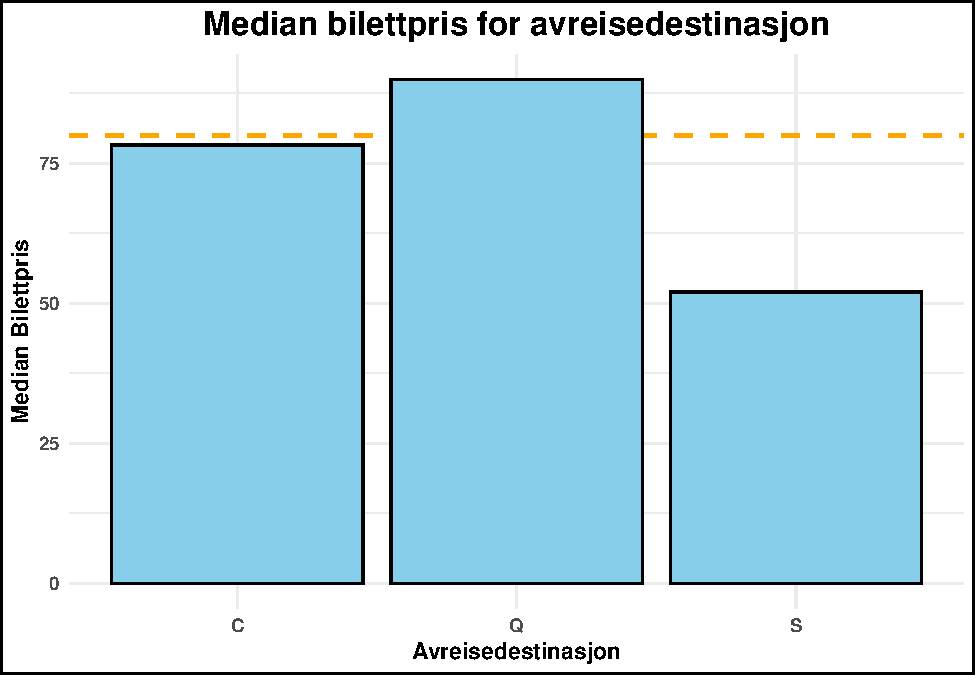
\includegraphics[width=0.8\linewidth]{presentation_files/figure-latex/unnamed-chunk-4-1} 

}

\caption{Pris for 1.klasse og avreisehavn.}\label{fig:unnamed-chunk-4}
\end{figure}

\subsubsection{Alder}\label{alder}

For passasjerer med manglende alder, bruker vi en median-alder som
standard, med en ekstra detalj for personer som reiste med søsken eller
ektefelle (SibSp \textgreater{} 0), men ikke med barn eller foreldre
(Parch == 0). I slike tilfeller bruker vi gjennomsnittsalderen for
personer med samme etternavn (antatt å være søsken eller ektefeller).
Dette gir mange av de reisende medianalder, men vi mener at ved å legge
til denne behandlingen vil vi kunne ha noe sterkere antakelser om
alderen til noen av passasjerene. Vi ser det kunne vært mulighet for at
andre faktorer kan påvirke alder, som f.eks. tittel eller klasse, men vi
har ikke tatt hensyn til dette i prosjektet.

\begin{Shaded}
\begin{Highlighting}[]
\NormalTok{handle\_na\_age }\OtherTok{\textless{}{-}} \ControlFlowTok{function}\NormalTok{(data) \{}
\NormalTok{  median\_age }\OtherTok{\textless{}{-}} \FunctionTok{median}\NormalTok{(data}\SpecialCharTok{$}\NormalTok{Age, }\AttributeTok{na.rm =} \ConstantTok{TRUE}\NormalTok{)}
\NormalTok{  data }\OtherTok{\textless{}{-}}\NormalTok{ data }\SpecialCharTok{\%\textgreater{}\%}
    \FunctionTok{mutate}\NormalTok{(}\AttributeTok{Age =} \FunctionTok{ifelse}\NormalTok{(}\FunctionTok{is.na}\NormalTok{(Age), }\FunctionTok{ifelse}\NormalTok{((SibSp }\SpecialCharTok{\textgreater{}} \DecValTok{0}\NormalTok{) }\SpecialCharTok{\&}\NormalTok{ (Parch }\SpecialCharTok{==} \DecValTok{0}\NormalTok{), }\FunctionTok{getSibSpAge}\NormalTok{(Name, data), median\_age), Age))}
  \FunctionTok{return}\NormalTok{(data)}
\NormalTok{\}}

\NormalTok{getSibSpAge }\OtherTok{\textless{}{-}} \ControlFlowTok{function}\NormalTok{(name, data) \{}
\NormalTok{  surname }\OtherTok{\textless{}{-}} \FunctionTok{get\_surname}\NormalTok{(name)}
  
\NormalTok{  sib\_sp }\OtherTok{\textless{}{-}} \FunctionTok{filter}\NormalTok{(}\FunctionTok{group\_by}\NormalTok{(data, Name), }\FunctionTok{get\_surname}\NormalTok{(Name) }\SpecialCharTok{==}\NormalTok{ surname)}
  
\NormalTok{  estimated\_age }\OtherTok{\textless{}{-}} \FunctionTok{round}\NormalTok{(}\FunctionTok{mean}\NormalTok{(sib\_sp}\SpecialCharTok{$}\NormalTok{Age, }\AttributeTok{na.rm =} \ConstantTok{TRUE}\NormalTok{))}
  \FunctionTok{return}\NormalTok{ (estimated\_age)}
\NormalTok{\}}

\NormalTok{get\_surname }\OtherTok{\textless{}{-}} \ControlFlowTok{function}\NormalTok{(name) \{}
\NormalTok{  surname }\OtherTok{\textless{}{-}} \FunctionTok{strsplit}\NormalTok{(name, }\StringTok{\textquotesingle{},\textquotesingle{}}\NormalTok{)[[}\DecValTok{1}\NormalTok{]][}\DecValTok{1}\NormalTok{]}
  \FunctionTok{return}\NormalTok{ (surname)}
\NormalTok{\}}
\end{Highlighting}
\end{Shaded}

\subsubsection{2. Ekstrahere tittel}\label{ekstrahere-tittel}

Vi ønsket å isolere tittelen fra navnet og legge den til i en egen
kolonne. Vår teori er at dette kan gjøre dataen mer tilpasset
maskinlæring ettersom tittelen kan være en indikator på faktorer som
sivilstatus, alder eller sosioøkonomisk status. Etter å ha testet
modellen og sjekket variabler innså vi at det var svært mange ulike
titler. Vi valgte derfor å håndtere dette ved å putte alle sjeldne
titler (\textless10) inn i en ``other'' varaibel.

\begin{figure}[H]

{\centering 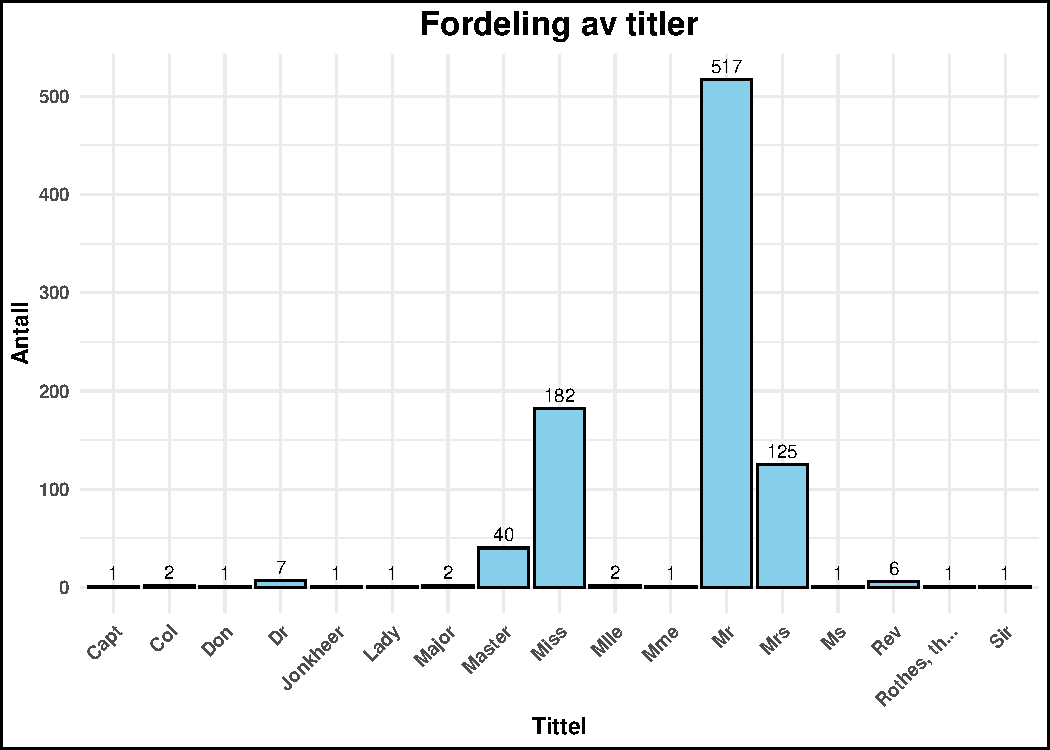
\includegraphics[width=0.8\linewidth]{presentation_files/figure-latex/unnamed-chunk-6-1} 

}

\caption{Antall passasjerer per tittel}\label{fig:unnamed-chunk-6}
\end{figure}

\subsubsection{3. Fjerne irrelevante og manglende
variabler}\label{fjerne-irrelevante-og-manglende-variabler}

For å redusere kompleksiteten i datasettet fjerner vi kolonnen Cabin
ettersom den har svært mange i datasettet som ikke hadde denne
variabelen. Vi så først på muligheten for at det var en tydelig
sammenheng mellom Pclass og Cabin ved bruk av en Chi-Squared. Det var
tydelig at passasjerer i Pclass 1 var konsentrert i A, B, C, D og E
kabiner, men ettersom det er svært lite data på hvor de resterende
reisende bodde, ville vi ikke gjøre noen generalisering rundt dette.
Name, Ticket og PassangerId er alle individuelle verdier som ikke vil ha
noen påvirkning på modellene så vi fjernet disse.

Gjennom hele data-wrangling prosessen sørger vi for at datasettet er
renere, mer konsistente og at de manglende variablene er håndtert.
Wranglingen kunne vært gjort på mange måter, og har en stor påvikning på
det endelige resultatet. Om vi skulle gjenntatt prosjektet burde vi i
større grad undersøkt datasettet i større grad før vi startet
wranglingen. Til tross for dette føler vi at dataen er håndtert på en
god måte.

\begin{figure}[H]

{\centering 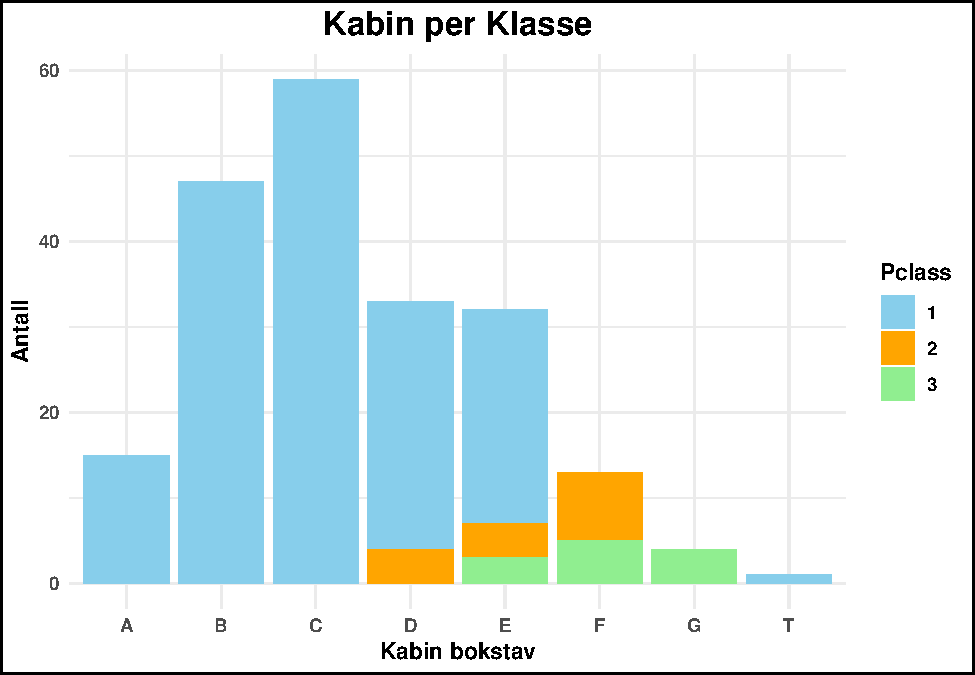
\includegraphics[width=0.8\linewidth]{presentation_files/figure-latex/unnamed-chunk-7-1} 

}

\caption{Kabin fordeling per klasse}\label{fig:unnamed-chunk-7}
\end{figure}

\subsubsection{Lag dummy-data og initial
split}\label{lag-dummy-data-og-initial-split}

\begin{Shaded}
\begin{Highlighting}[]
\NormalTok{model\_data }\OtherTok{\textless{}{-}} \FunctionTok{create\_dummy\_data}\NormalTok{(data)}
\NormalTok{t\_train }\OtherTok{\textless{}{-}}\NormalTok{ model\_data}\SpecialCharTok{$}\NormalTok{t\_train}
\NormalTok{t\_test }\OtherTok{\textless{}{-}}\NormalTok{ model\_data}\SpecialCharTok{$}\NormalTok{t\_test}
\end{Highlighting}
\end{Shaded}

\subsubsection{Tren modeller}\label{tren-modeller}

Vi fant ut at de mest relevant modellene for problemet var Lasso, Random
Forest og Gradient Boosting Tree. Her implementerer vi dem, og finner de
beste hyperparameterne. Vi laget en funksjon som tar inn modelnavn som
parameter, og utifra navnet lager den en modelspesifikkasjon samt en
grid med potensielle hyperparameter. Spennet av verdier i dette griddet
har vi valgt basert på det som virker som konsensus på blant annet Stack
Overflow. Videre bruker den tune\_grid() fra tune-biblioteket i
Tidyverse i kombinasjon med select\_best() til å finne hvilke
hyperparametere som sammen gir den beste treffsikkerheten.

\begin{Shaded}
\begin{Highlighting}[]
\CommentTok{\# Tuned models}
\NormalTok{tuned\_lso }\OtherTok{\textless{}{-}} \FunctionTok{create\_tuned\_model}\NormalTok{(}\StringTok{"lasso"}\NormalTok{, t\_train) }
\NormalTok{tuned\_rf }\OtherTok{\textless{}{-}} \FunctionTok{create\_tuned\_model}\NormalTok{(}\StringTok{"random\_forest"}\NormalTok{, t\_train) }
\NormalTok{tuned\_xgb }\OtherTok{\textless{}{-}} \FunctionTok{create\_tuned\_model}\NormalTok{(}\StringTok{"xgboost"}\NormalTok{, t\_train) }
\end{Highlighting}
\end{Shaded}

Deretter trener vi modellene og undersøker treffsikkerheten deres i å
avgjøre hvem som overlever.

\begin{Shaded}
\begin{Highlighting}[]
\NormalTok{lso\_fit }\OtherTok{\textless{}{-}}\NormalTok{ tuned\_lso }\SpecialCharTok{\%\textgreater{}\%}
  \FunctionTok{fit}\NormalTok{(Survived }\SpecialCharTok{\textasciitilde{}}\NormalTok{., }\AttributeTok{data =}\NormalTok{ t\_train)}
\NormalTok{rf\_fit }\OtherTok{\textless{}{-}}\NormalTok{ tuned\_rf }\SpecialCharTok{\%\textgreater{}\%}
  \FunctionTok{fit}\NormalTok{(Survived }\SpecialCharTok{\textasciitilde{}}\NormalTok{., }\AttributeTok{data =}\NormalTok{ t\_train)}
\NormalTok{xgb\_fit }\OtherTok{\textless{}{-}}\NormalTok{ tuned\_xgb }\SpecialCharTok{\%\textgreater{}\%} 
  \FunctionTok{fit}\NormalTok{(Survived }\SpecialCharTok{\textasciitilde{}}\NormalTok{., }\AttributeTok{data =}\NormalTok{ t\_train)}

\NormalTok{tuned\_lso\_pred }\OtherTok{\textless{}{-}} \FunctionTok{predict}\NormalTok{(lso\_fit, }\AttributeTok{new\_data =}\NormalTok{ t\_test, }\AttributeTok{type =} \StringTok{"class"}\NormalTok{)}\SpecialCharTok{$}\NormalTok{.pred\_class}
\NormalTok{tuned\_rf\_pred }\OtherTok{\textless{}{-}} \FunctionTok{predict}\NormalTok{(rf\_fit, }\AttributeTok{new\_data =}\NormalTok{ t\_test, }\AttributeTok{type =} \StringTok{"class"}\NormalTok{)}\SpecialCharTok{$}\NormalTok{.pred\_class}
\NormalTok{tuned\_xgb\_pred }\OtherTok{\textless{}{-}} \FunctionTok{predict}\NormalTok{(xgb\_fit, }\AttributeTok{new\_data =}\NormalTok{ t\_test, }\AttributeTok{type =} \StringTok{"class"}\NormalTok{)}\SpecialCharTok{$}\NormalTok{.pred\_class}

\NormalTok{tuned\_lso\_acc }\OtherTok{\textless{}{-}} \FunctionTok{mean}\NormalTok{(tuned\_lso\_pred }\SpecialCharTok{==}\NormalTok{ t\_test}\SpecialCharTok{$}\NormalTok{Survived)}
\NormalTok{tuned\_rf\_acc }\OtherTok{\textless{}{-}} \FunctionTok{mean}\NormalTok{(tuned\_rf\_pred }\SpecialCharTok{==}\NormalTok{ t\_test}\SpecialCharTok{$}\NormalTok{Survived)}
\NormalTok{tuned\_xgb\_acc }\OtherTok{\textless{}{-}} \FunctionTok{mean}\NormalTok{(tuned\_xgb\_pred }\SpecialCharTok{==}\NormalTok{ t\_test}\SpecialCharTok{$}\NormalTok{Survived)}


\NormalTok{accs }\OtherTok{\textless{}{-}} \FunctionTok{tibble}\NormalTok{ (}
  \AttributeTok{Model =} \FunctionTok{c}\NormalTok{(}\StringTok{"LASSO"}\NormalTok{, }\StringTok{"RANDOM FOREST"}\NormalTok{, }\StringTok{"XGBOOST"}\NormalTok{),}
  \AttributeTok{Treffsikkerhet =} \FunctionTok{c}\NormalTok{(tuned\_lso\_acc, tuned\_rf\_acc, tuned\_xgb\_acc) }\CommentTok{\#code in Norwegian because knitr::kable uses }
\NormalTok{)}

\NormalTok{knitr}\SpecialCharTok{::}\FunctionTok{kable}\NormalTok{(accs, }\AttributeTok{caption =} \StringTok{"Nøyaktighet for ulike modeller"}\NormalTok{)}
\end{Highlighting}
\end{Shaded}

\begin{longtable}[]{@{}lr@{}}
\caption{Nøyaktighet for ulike modeller}\tabularnewline
\toprule\noalign{}
Model & Treffsikkerhet \\
\midrule\noalign{}
\endfirsthead
\toprule\noalign{}
Model & Treffsikkerhet \\
\midrule\noalign{}
\endhead
\bottomrule\noalign{}
\endlastfoot
LASSO & 0.8491620 \\
RANDOM FOREST & 0.8547486 \\
XGBOOST & 0.8324022 \\
\end{longtable}

Modellene har relativt lik treffsikkerhet. Ca. 85\% er ikke - isolert
sett - særlig imponerende. Vi tror likevel dette er omtrent hvor
treffsikker en slik model kan bli gitt problemstillingen samt hvor lite
datasettet er. Vi kommer tilbake til dette i siste avsnitt.

\subsubsection{Hvilke faktorer påvirker resultatet
mest}\label{hvilke-faktorer-puxe5virker-resultatet-mest}

Videre ønsker vi å se på hvilken innvirkning hver enkelt faktor har på
de ulike modellene. Gradient Boosting Tree fokuserte i stor grad på et
fåtall variabler. Vi valge derfor å fremstille den i et eget plot.
Vip-biblioteket ble brukt til å finne de viktigste faktorene.

\begin{figure}[H]

{\centering 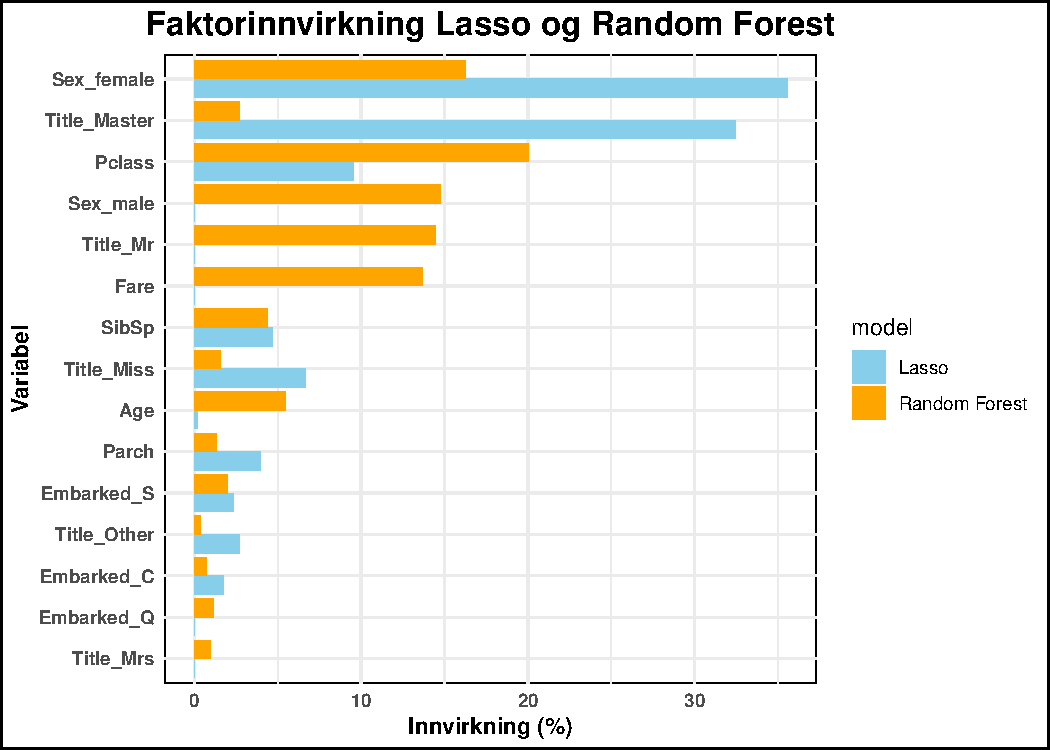
\includegraphics[width=0.8\linewidth]{presentation_files/figure-latex/unnamed-chunk-11-1} 

}

\caption{Faktorinnvirkning Lasso og Random Forrest}\label{fig:unnamed-chunk-11}
\end{figure}

\begin{figure}[H]

{\centering 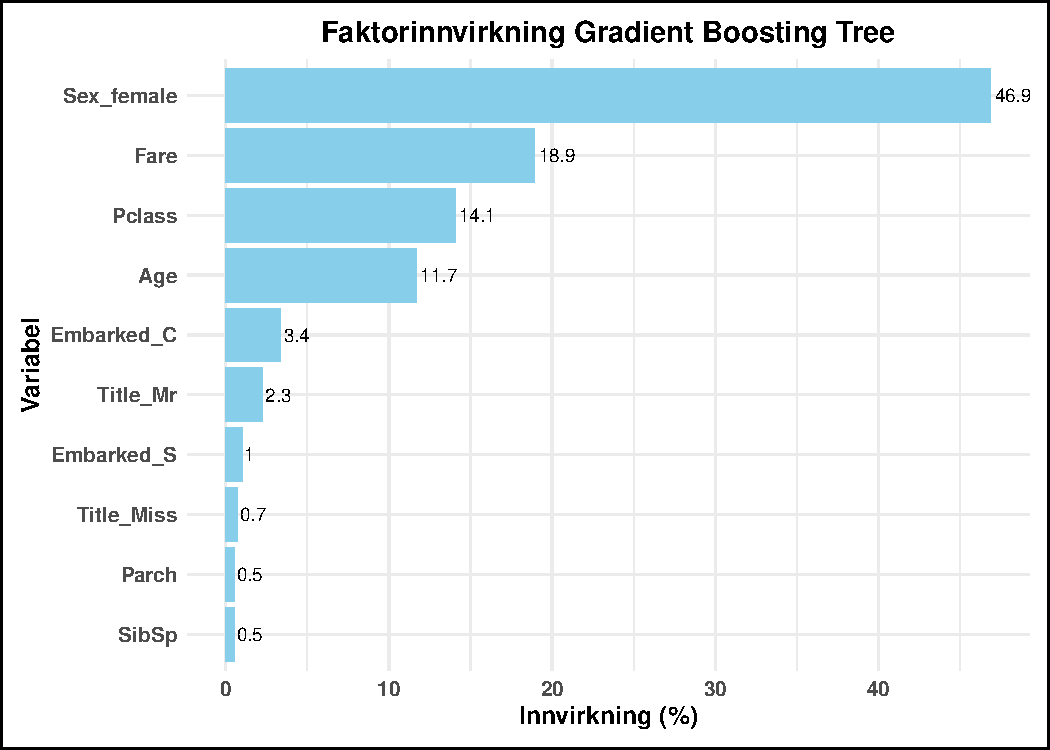
\includegraphics[width=0.8\linewidth]{presentation_files/figure-latex/unnamed-chunk-12-1} 

}

\caption{Faktorinnvirkning XGB}\label{fig:unnamed-chunk-12}
\end{figure}

\section{}\label{section}

Vi ser at de forskjellige modellene vektlegger forskjellige faktorer.
Dette ser ut til å gjelde også når vi ikke bruker set.seed(). Dette
stammer trolig fra at modellene gjennomfører treningen forskjellig,
spesielt mellom de tre-baserte modellene og Lasso.

Et resultat som er spesielt interessant ifra disse figurene er hvor lite
viktighet Lasso gir til faktorer som blant annet sex\_male, title\_mr.
Disse faktorene forteller oss at passasjerene er menn, noe som er
avdekket i studier til å være en av de viktigste faktorene. Likevell har
to av modellene ingen fokus på dem. Vi konkluderer med at dette er fordi
sex\_female - som samtlige modeller har satt mye fokus på - forteller
modellen nok om hvilket kjønn passasjeren har. Dette er spesielt aktuelt
i Lasso, hvor en av karakteristikkene er å straffe bruk av koeffisienter
eller veldig sammenhengende faktorer, men vi ser det også i Gradient
Boosting Tree.

\subsubsection{Brukergrensesnitt}\label{brukergrensesnitt}

I brukergrensesnittet har vi implementert mulighet for en bruker å
«kjøpe en billett» til Titanic. Når dataen er samlet inn bruker vi
informasjonen i modellen for å forutsi om brukeren ville overlevd
forliset eller ikke. Vi benyttet biblioteket «shiny» for å lage
grensesnittet. Informasjonen vi henter fra brukeren er:

\begin{enumerate}
\def\labelenumi{\arabic{enumi}.}
\tightlist
\item
  All relevant informasjon for modellen. Tittel, alder, kjønn,
  avreisested, billettklasse og om man reiser med søsken, barn,
  ektefelle eller foreldre.
\item
  Grensesnittet ber også om brukerens navn til tross for at det er
  individuelle verdier som ikke benyttes i modellen. Dette gjør vi
  ettersom vi mener det gir en mer realistisk brukeropplevelse.
\end{enumerate}

\subsubsection{Håndtering av data i
grensesnitt}\label{huxe5ndtering-av-data-i-grensesnitt}

Planen fra starten av wranglingen i grensesnittet var å lage en tibble
som matchet det råe datasettet slik at vi kunne sende denne dataen inn i
wrangling.R og videre inn i model\_data.R for å gjøre dataen klar for
modellen. Vi innså dog at det hadde dukket opp noe teknisk gjeld, med
kun noen dager igjen til prosjektet skulle leveres.

Model\_data.R, som håndterte dataen og lagde dummydata splittet også opp
dataen i treningsdata og testdata. Vi så på muligheten for å splitte opp
denne funksjonen, men når vi kjørte ``bake'' på den nye dataen med kun
en rad fungerte ikke dette, ettersom ``bake'' ikke kan opprette alle
dummy-variablene vi trengte. Ettersom grensesnittet kun besto av en rad
med data og skulle håndteres av en ferdig trent modell var vi nødt til å
finne en rask nødløsning.

Vi håndterte dette ved å manuelt opprette en tibble som matchet dataen -
etter den var prosessert av model\_data - i serversiden av appen. Disse
valgene ble tatt, delvis grunnet miskommunikasjon og oppdeling av
oppgaver. Vi ser at dette muligvis kunne blitt gjort på en både bedre og
enklere måte om vi skulle jobbet videre på prosjektet.

Billettprisen er en faktor i modellen, men noe vi ikke så på som særlig
relevant for grensesnittet. Vi valgte derfor å finne medianprisen for
hver enkelt avreisehavn og billettklasse og på den måten sette en pris
basert på ``billetten man kjøper''. Resultatet av dette er nå hardkodet
inn i app.R

\begin{figure}[H]

{\centering 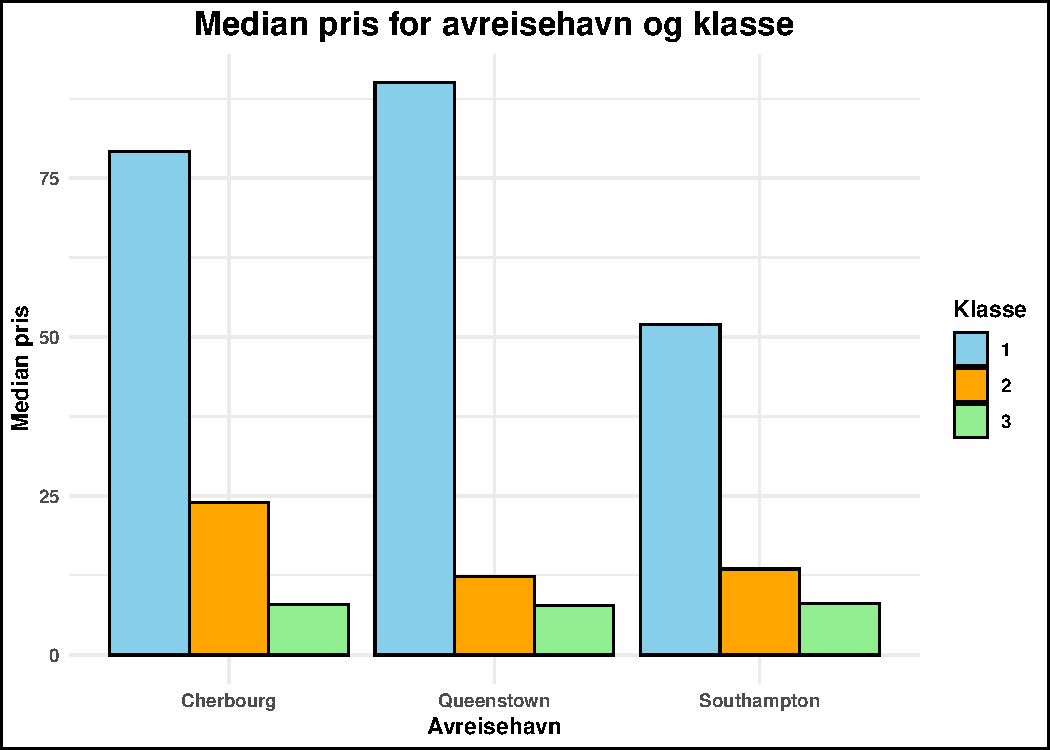
\includegraphics[width=0.8\linewidth]{presentation_files/figure-latex/unnamed-chunk-13-1} 

}

\caption{Pris for klasse og avreisedestinasjon.}\label{fig:unnamed-chunk-13}
\end{figure}

Vi har også noen globale variabler i prosjektet som vi ble nødt til å
bruke grunnet mangel på tid og erfaring med utvikling av grensesnitt og
shiny pakken i R.

Grensesnittet bruker ferdig trente modeller lagret med saveRDS og hentet
med readRDS. Dette ønsket vi å gjøre slik at grensesnittet ikke trenger
å vente på trening av modeller for hver gang man benytter det.

\subsubsection{Resultat}\label{resultat}

Når brukeren trykker på «Kjøp billett» knappen vil dataen transformeres
og den lagrede modellen blir kjørt på dataen fra brukeren. Grensesnittet
viser umiddelbart indikasjonen fra modellen om brukeren ville overlevd
forliset eller ikke.

\subsubsection{Oppsummering og
refleksjon}\label{oppsummering-og-refleksjon}

I dette prosjektet har vi jobbet med å bygge en maskinlæringsmodell for
å forutsi overlevelse på Titanic ved å analysere passasjerdata. Mye av
arbeidet gikk med til å rense og forbedre dataen. Vi ser på det som
svært sannsynlig at mye av modellenes treffsikkerhet ligger i dette
steget.

Ettersom dette er en kjent oppgave, med mange tidligere gode løsninger
var vi opptatt av å ikke gjøre noen research på forhånd på hvordan andre
har løst problemet. Vi ønsket å løse oppgaven på best mulig måte uten
hjelp eller inspirasjon fra andre løsninger. Etter å ha gjennomført vår
beste løsning har vi dog sett at andre har klart å løse problemet med
høyere treffsikkerhet.

En grunn til viktigheten av wrangling prosessen er størrelsen på
datasettet. Med kun ca. 900 rader med data gjør det viktigheten av å
håndtere manglende data på en god måte svært verdifullt. For hver
variabel man tar ut av settet, eller setter unøyaktige verdier vil
modellen ha et dårligere grunnlag for å gjøre nøyaktige prediksjoner.

Vi mener fremdeles at vi har gjort en god innsats med å forberede dataen
til vår evne. Selv om vi nå - med vår nye læring og kunnskap - ser at
det er forbedringer vi kunne gjort.

Inkluderingen av et grensesnitt er noe som gir oppgaven et preg av
interaktivitet, som vi synes er et spennende tillegskomponent. Å kunne
benytte modellen og gjøre den tilgjengelig for brukere og gi en
prediksjon for overlevelse gir prosjektet et mer praktisk og
engasjerende aspekt. Til tross for mangel på erfaring med utvikling av
grensesnitt, samt noen raske nødløsninger, synes vi at det fungerer
godt.

Til tross for forbedringspotensialet er vi fornøyd med hva vi har
oppnådd. Vi har fått en bedre forståelse for maskinlæring, og kanskje
særlig viktigheten av å håndtere dataen på en god måte.

\end{document}
